%\clearpage
\section{Event and Object Selection}
\label{sec:selection}

\par At preselection, events must pass an OR of 
\verb% EF_e24vhi_medium1%, \verb% EF_mu24i_tight%,\\
\verb% EF_e60_medium1%, \verb% EF_mu36_tight%, 
\verb% EF_e12Tvh_medium1_mu8%, 
 \verb% EF_mu18_tight_mu8_EFFS% and \verb% EF_2e12Tvh_loose1%
 to get considered for analysis. They must also have exactly two leptons 
with $\pt>15$~\GeV. A reconstructed primary vertex is not required to have 
a minimum number of tracks associated with it.  
All other preselection cuts are identical to those used for the 
\HWW\ study in Ref.~\cite{ATLASCONF2014060}. 

\par The electron identification criteria closely follows the 
 standard \HWW\ selection which relies on a likelihood-based method to
identify electrons from electromagnetic (EM) showers and Inner Detector (ID) tracks. 
A more detailed description of this method can be found in Ref. ~\cite{ATLASCONF2014060}.
EM showers and ID tracks are required to have $\pt > 15$~\GeV and lie in 
pseudorapidity less than 2.47 and out of the detector crack 
( [1.37,1.52]). Electron candidates with $15<\pt<25$~\GeV have to satisfy the very tight 
likelihood requirement and those with $\pt>25$~\GeV have to satisfy the medium 
likelihood requirement. This is because the latter are less likely to be misidentified 
objects. Calorimeter isolation is also imposed on electron 
objects by considering the energy deposited in a cone of $\Delta R = 0.3$ 
around the electron object cluster. Track isolation is also considered by taking 
the sum \pt\ of all the tracks with $\pt>400$~\MeV\ within a cone 
of size $\Delta R = 0.3$. To separate these electron objects from prompt 
electrons, impact parameter variables are used.  

\begin{figure}[!h]
\centering
\begin{tabular}{c}
	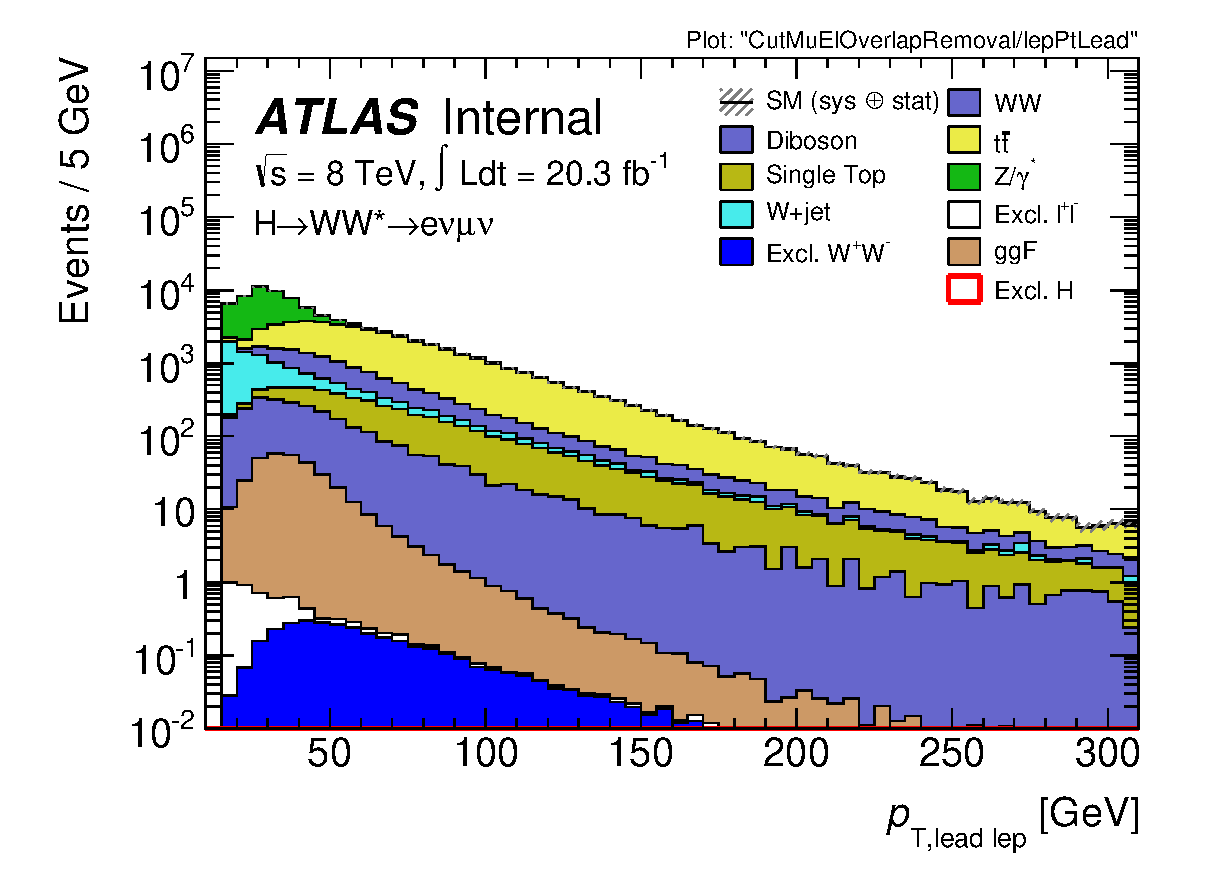
\includegraphics[width=0.5\linewidth]{em_CutMuElOverlapRemoval_lepPtLead_mh125_log.eps}
	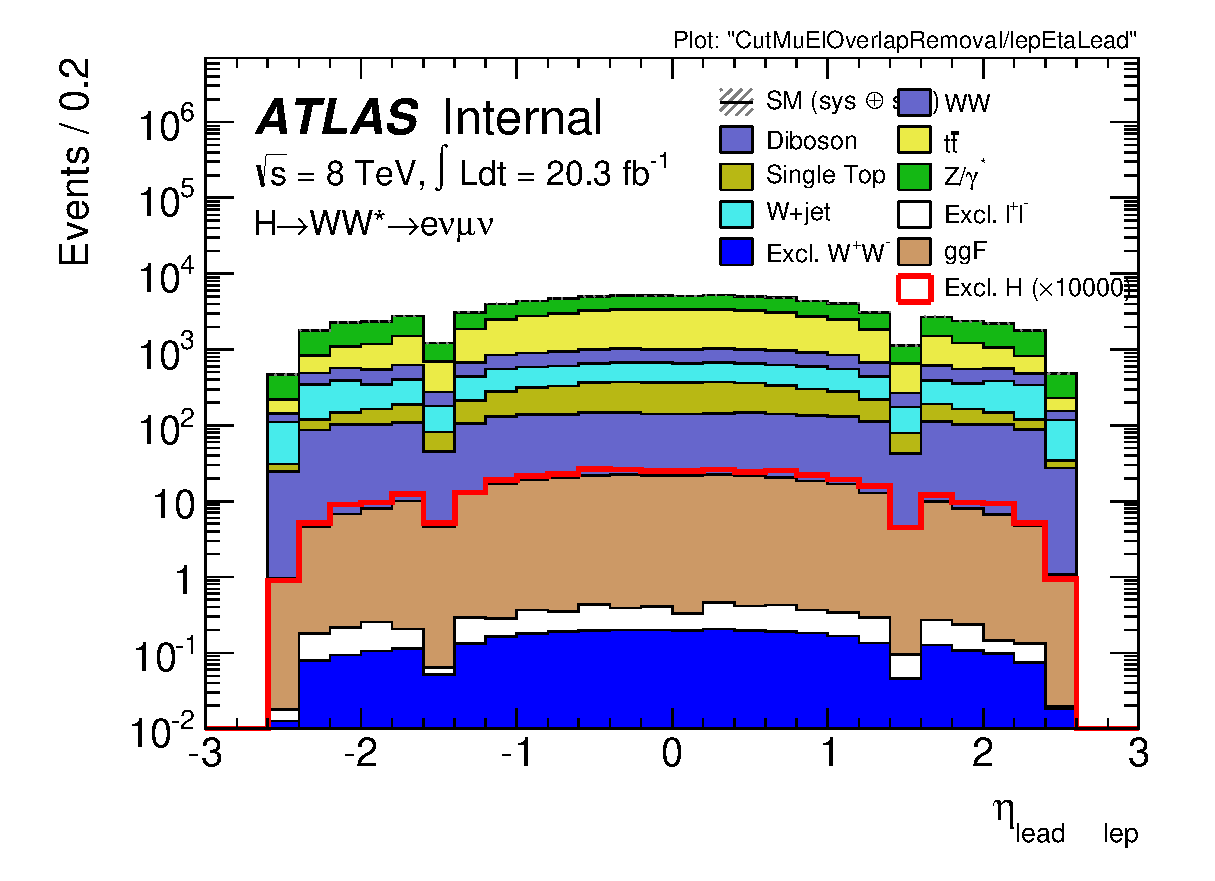
\includegraphics[width=0.5\linewidth]{em_CutMuElOverlapRemoval_lepEtaLead_mh125_log.eps}\\
\end{tabular}
\caption{Electron distributions}
\label{fig:electrons}
\end{figure}
%
\par Candidates for muon objects should be objects with matched hits from the ID and the 
Muon Spectrometer (MS). The algorithms that match ID tracks to MS tracks are described 
in detail in Ref.~\cite{Aad2014rra}. These objects are further required to have 
$\pt > 15$~\GeV\ and must lie within pseudorapidity of 2.47.
The sum of the pixel hits and dead sensors should be at least 1.
The sum of sct hits and dead sensors should also be at least 5.  

\begin{figure}[!h]
\centering
\begin{tabular}{c}
	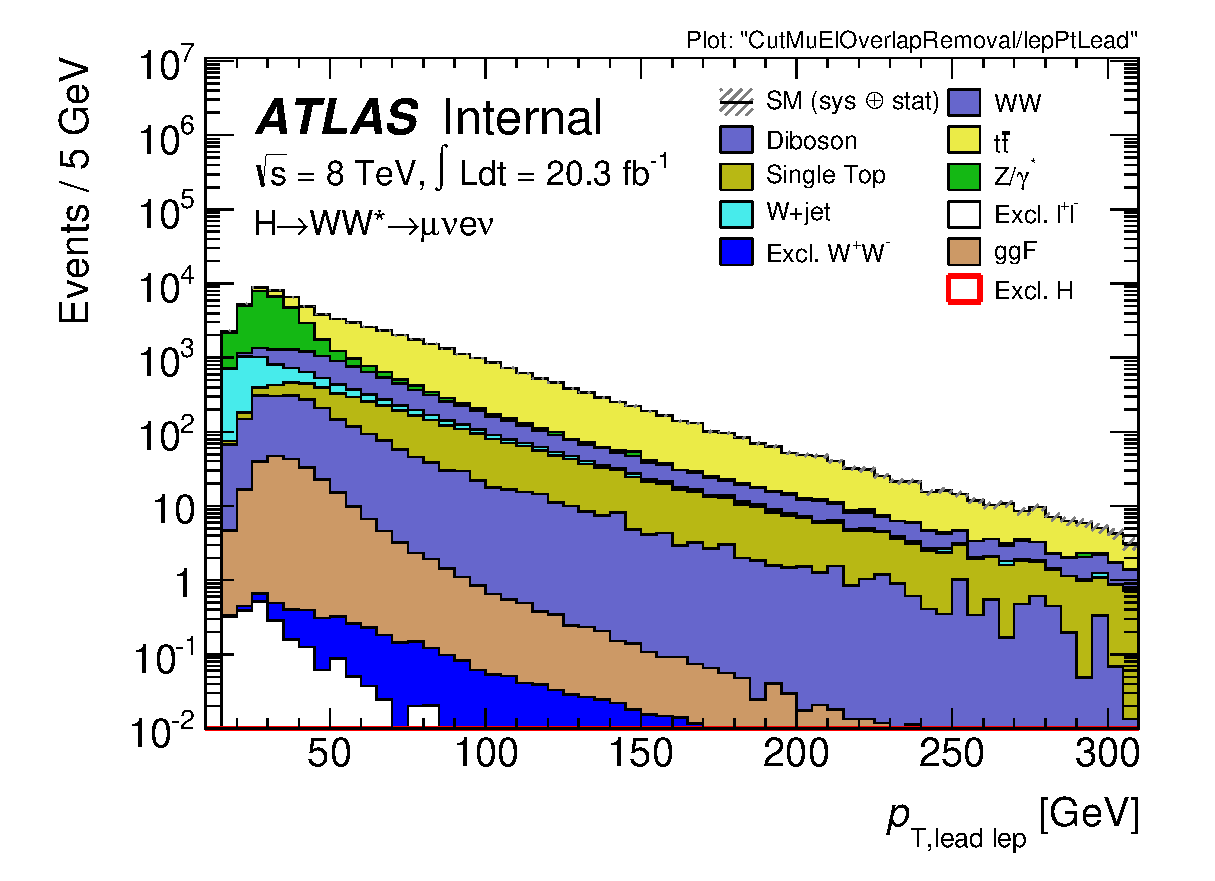
\includegraphics[width=0.5\linewidth]{me_CutMuElOverlapRemoval_lepPtLead_mh125_log.eps}
	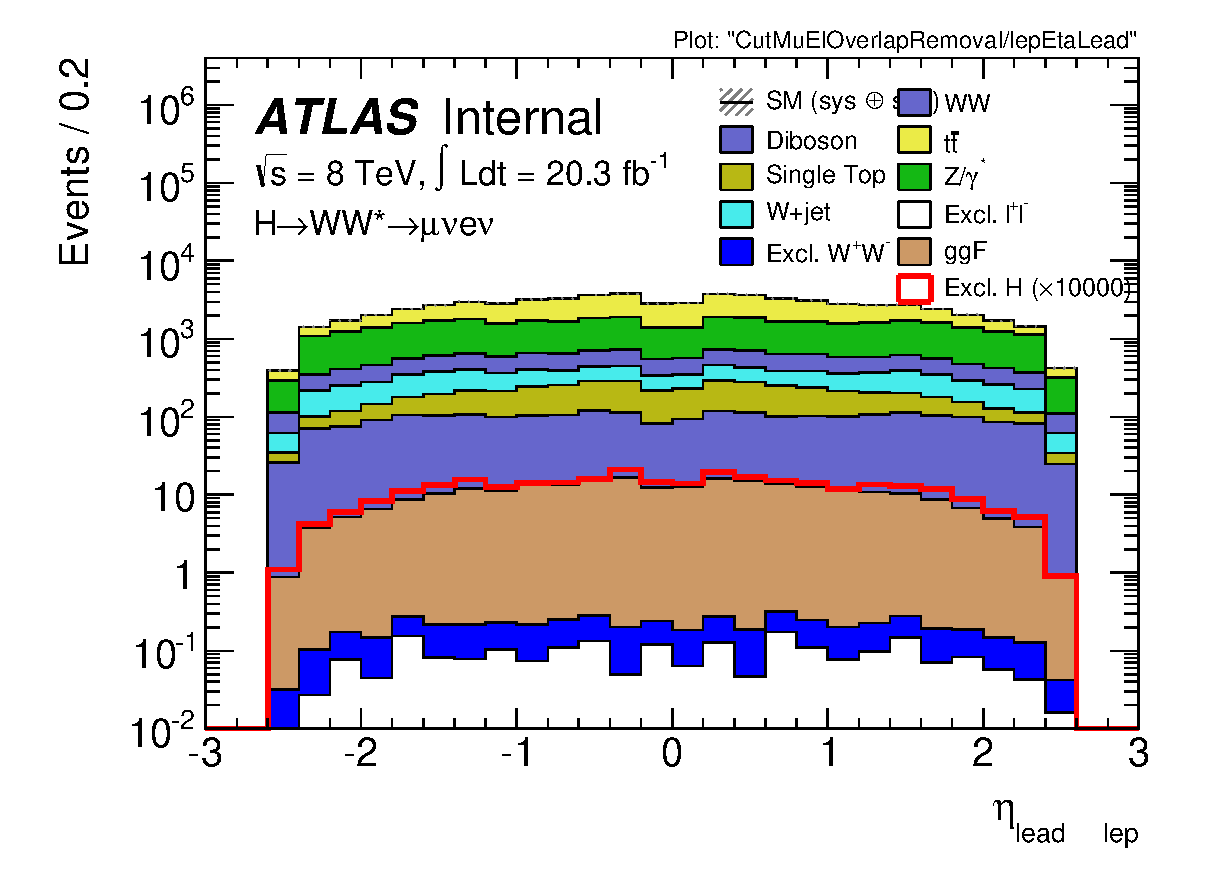
\includegraphics[width=0.5\linewidth]{me_CutMuElOverlapRemoval_lepEtaLead_mh125_log.eps}\\
\end{tabular}
\caption{Muon distributions}
\label{fig:muons}
\end{figure}

\par Tracks are required to have at least 1 pixel hit and at least 4 sct hits and 
have at least 400 MeV \pt. They are also required to be within $|\eta|<2.47$.

\begin{figure}[!h]
\centering
	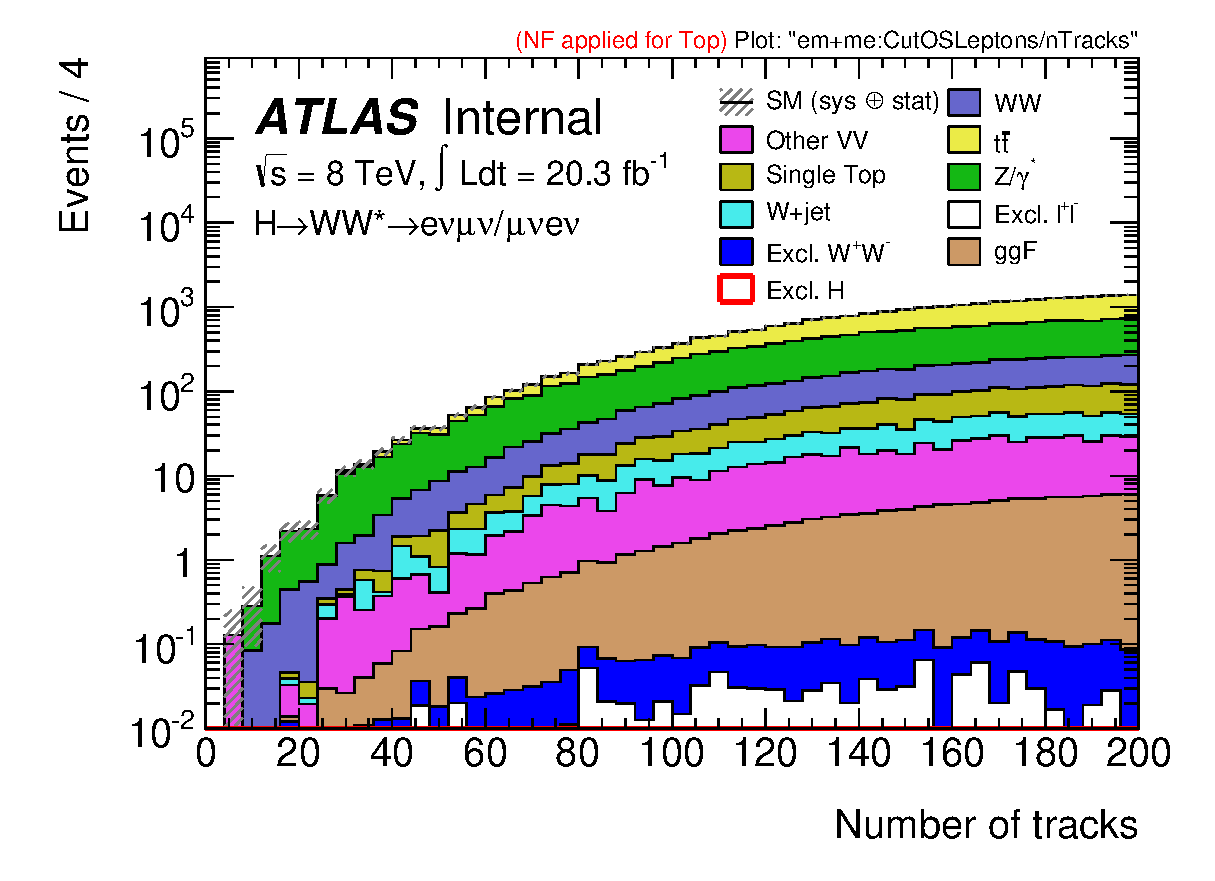
\includegraphics[width=0.5\linewidth]{emme_CutOSLeptons_nTracks_mh125_log.eps}\\
\caption{Number of selected tracks}
\label{fig:nTracks.}
\end{figure}

\par The signal region for events that pass the pre-selection criteria is carefully 
designed to select events with Higgs properties. An exclusivity requirement is further imposed.
The lepton with higher \pt\ is required to have $\pt>25$ GeV. This will be refered to as the 'leading 
lepton'. The second lepton, with lower \pt\ is required to have $\pt>15$ GeV. It will 
be refered to as the 'sub-leading lepton'. The high \pt\ selection on the leptons  is 
meant to reduce W+jets and QCD multi-jets backgrounds, where low-\pt\ jets are 
mis-identified as leptons. To exploit the fact that the SM Higgs is neutral, the 
leading and sub-leading leptons are required to be of opposite sign. This cut will be refered to 
as 'OS Leptons' in this note. 
\par The invariant mass of the dilepton system \mll, is demanded to 
be fall within 10 GeV and 55 GeV. The reason for a lower bound is that 
some of the backgrounds such at Z+jets are not modelled correctly at low \mll. In this analysis
only Z+jets MC samples generated at $\mll>10$ GeV are used. Figure~\ref{fig:mllOSLeptons}
shows the \mll\ distribution for events that pass the preselection cuts, lepton \pt\ cuts
and the opposite sign requirement on the leptons. The $\mll>10$ GeV cut yields a 
signal survival efficiency of 98\%. Figure~\ref{fig:mllOSLeptons} also justifies an upper bound on 
\mll\ for Higgs events. Since the Higgs boson is of spin zero, \mll\ tends to peak at lower
 values than for the WW backgrounds. A $\mll<55$ GeV cut rejects 75\% of inclusive WW background 
and keeps 86\% of signal. 

\begin{figure}[!h]
\centering
	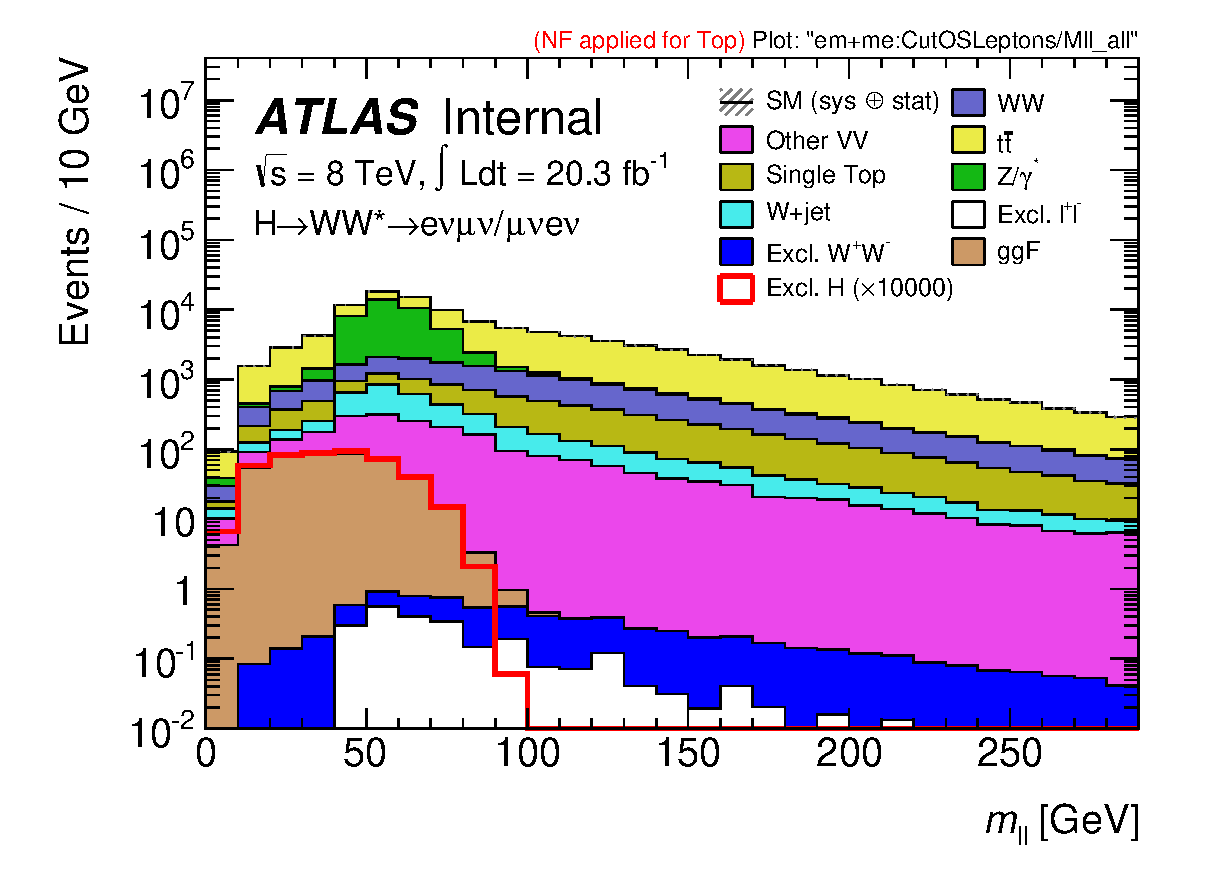
\includegraphics[width=0.5\linewidth]{emme_CutOSLeptons_Mll_all_mh125_log.eps}\\
\caption{\mll\ distribution for signal (scaled by $10^4$) and relevant backgrounds for 
events that pass preselection, lepton \pt, and OS lepton cuts. Z+jets are not well modelled 
for $\mll<10$ GeV, so we consider events with $\mll>10$ GeV. Signal survival after this cut 
is 98\%. An $\mll<55$ GeV cut further rejects 75\% of WW background while keeping 86\% of signal.}
\label{fig:mllOSleptons}
\end{figure}

\par The neutrinos in the signal final state are identified by a momentum imbalance in the detector.
This imbalance is quantified by the variable 'missing transverse momentum',
\met\ that is calculated as 

\begin{equation}
\met = - \left (\sum_{selected}\pt + \sum_{soft}\pt \right )
\end{equation}   

where $\sum_{selected}\pt$ is the vectorial sum of \pt\ from 
all the objects identified by ATLAS identification 
algorithms, such as leptons, photons and jets. In this analysis these 
objects are required to have $\pt>20$ GeV. $\sum_{selected}\pt$ is the vectorial sum 
of \pt\ from all other objects that have low values of \pt, extracted 
from tracks with $\pt>0.5$ GeV that originate from the primary vertex. 
Both \met and its relative direction to leptons and jets are effective variables 
in rejecting Drell-Yan \tautau\ background, where \met\ 
aligns with a final state lepton. A special variable, \metRel (see Ref.~\cite{ATLASCONF2014060} for 
a more detailed description of this variable) is used to quantify how close in the transverse 
plane \met\ is to leptons and jets:

\begin{equation}
\metRel = \begin{cases}
				 \met\sin\Delta\phi_{near} & \text{if $\Delta\phi_{near}<\pi/2$} \\
				 \met & \text{otherwise,}
					\end{cases}
\end{equation}  

where $\Delta\phi_{near}$ is the azimuthal separation of the \met\ and the nearest 
high-\pt jet or lepton. Figure ... shows ...

show plot of METRel.... it should prove that Ztautau is reduced by cutting on it.  

\begin{figure}[!h]
\centering
\begin{tabular}{c}
	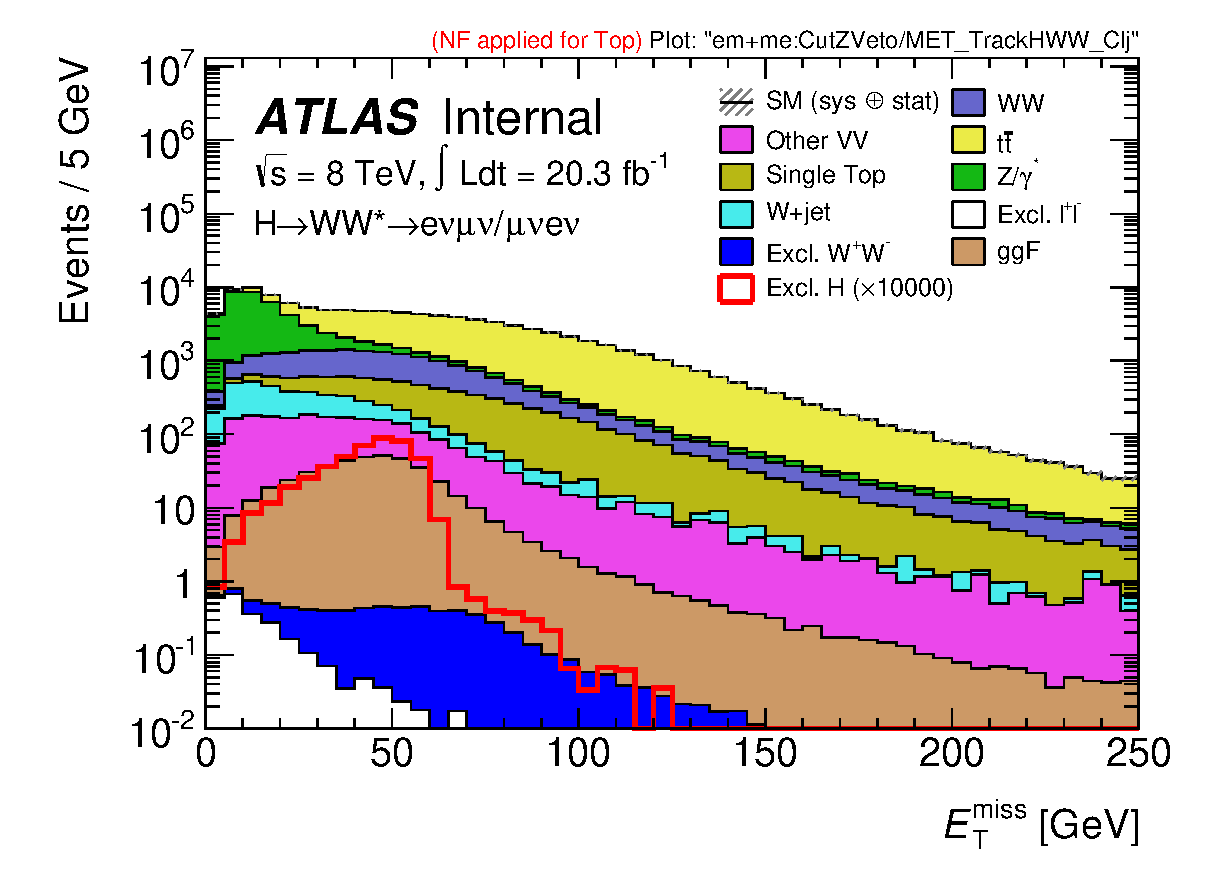
\includegraphics[width=0.5\linewidth]{emme_CutZVeto_MET_TrackHWW_Clj_mh125_log.eps}
	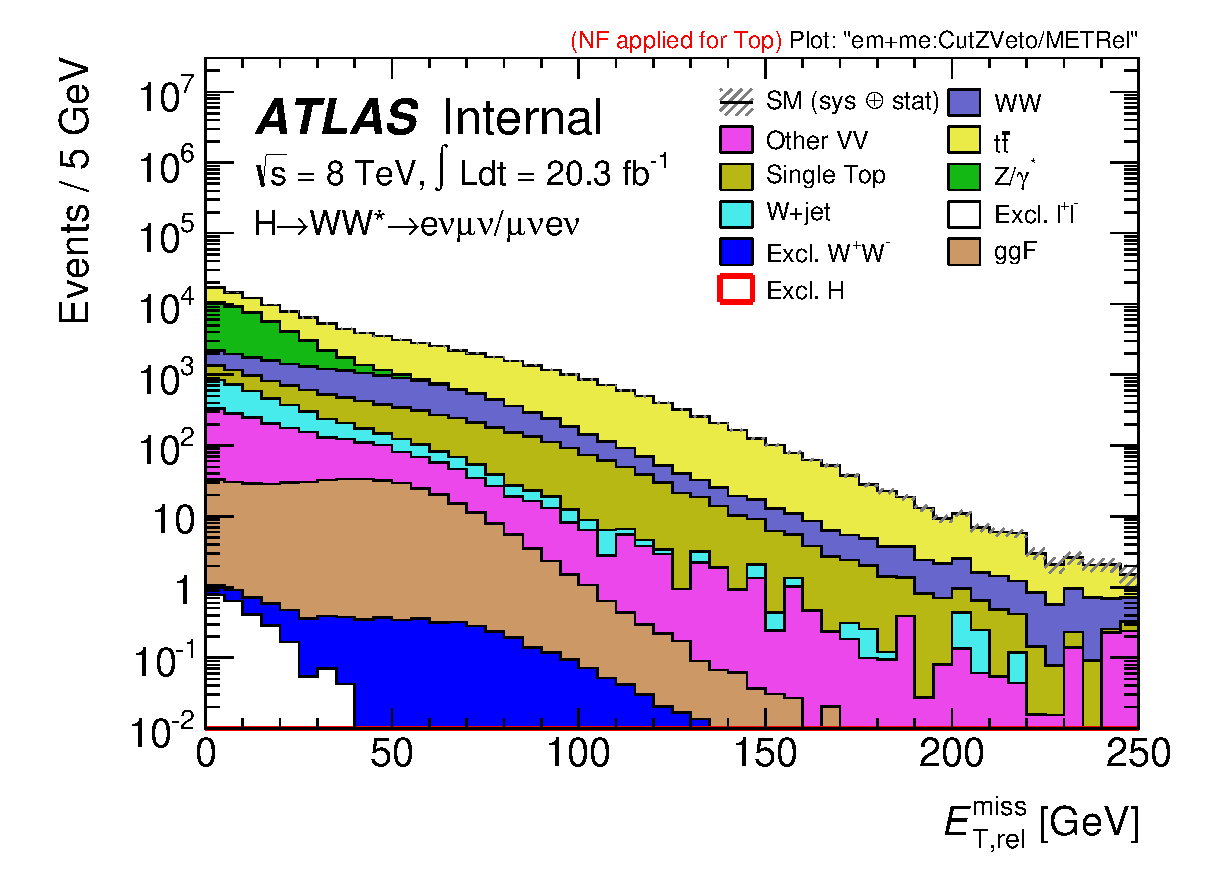
\includegraphics[width=0.5\linewidth]{emme_CutZVeto_METRel_mh125_log.eps}\\
\end{tabular}
\caption{Talk about MET selection}
\label{fig:met}
\end{figure}

\par 
talk about dphillmet and add a plot....
\begin{figure}[!h]
\centering
	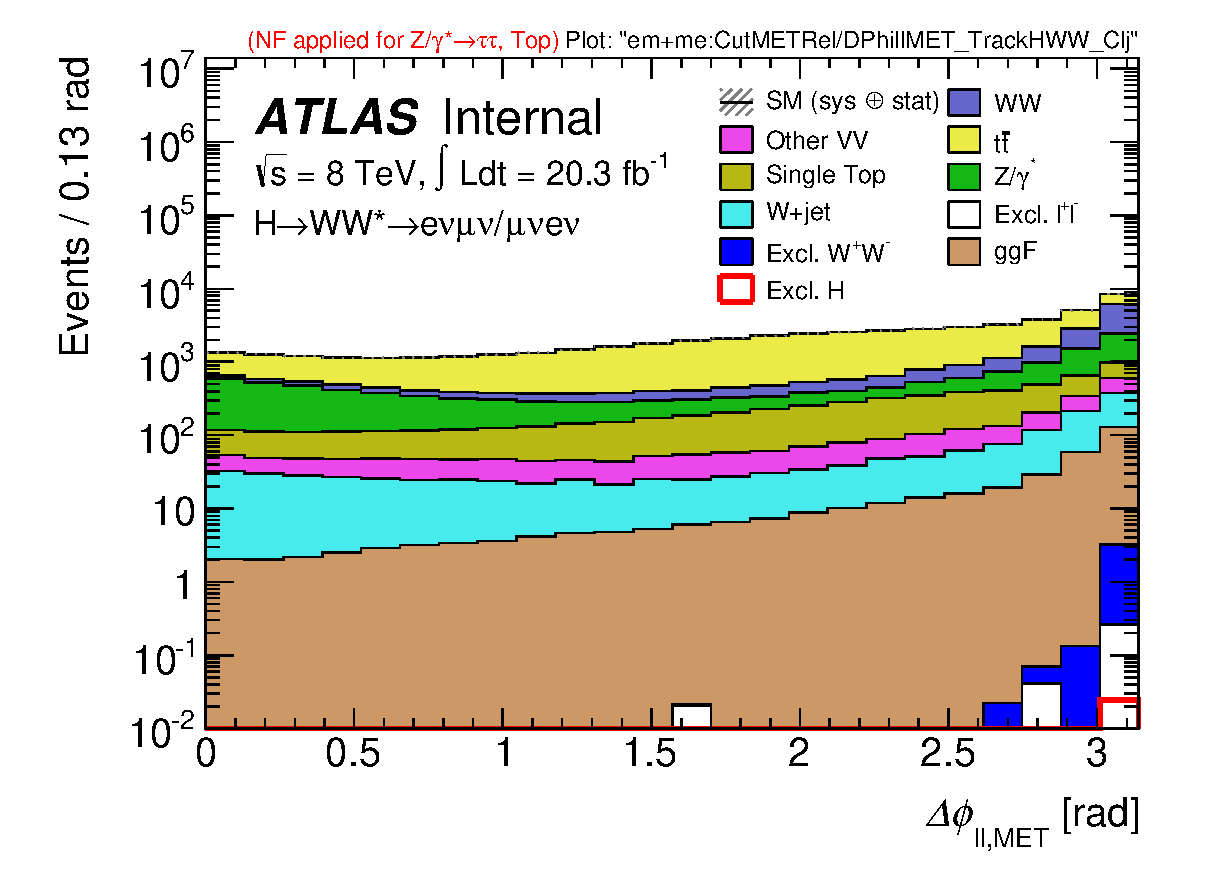
\includegraphics[width=0.5\linewidth]{emme_CutMETRel_DPhillMET_TrackHWW_Clj_mh125_log.eps}\\
\caption{dphillmet}
\label{fig:dphillmet}
\end{figure}

\par 
talk about ptll and add a plot ...
\begin{figure}[!h]
\centering
	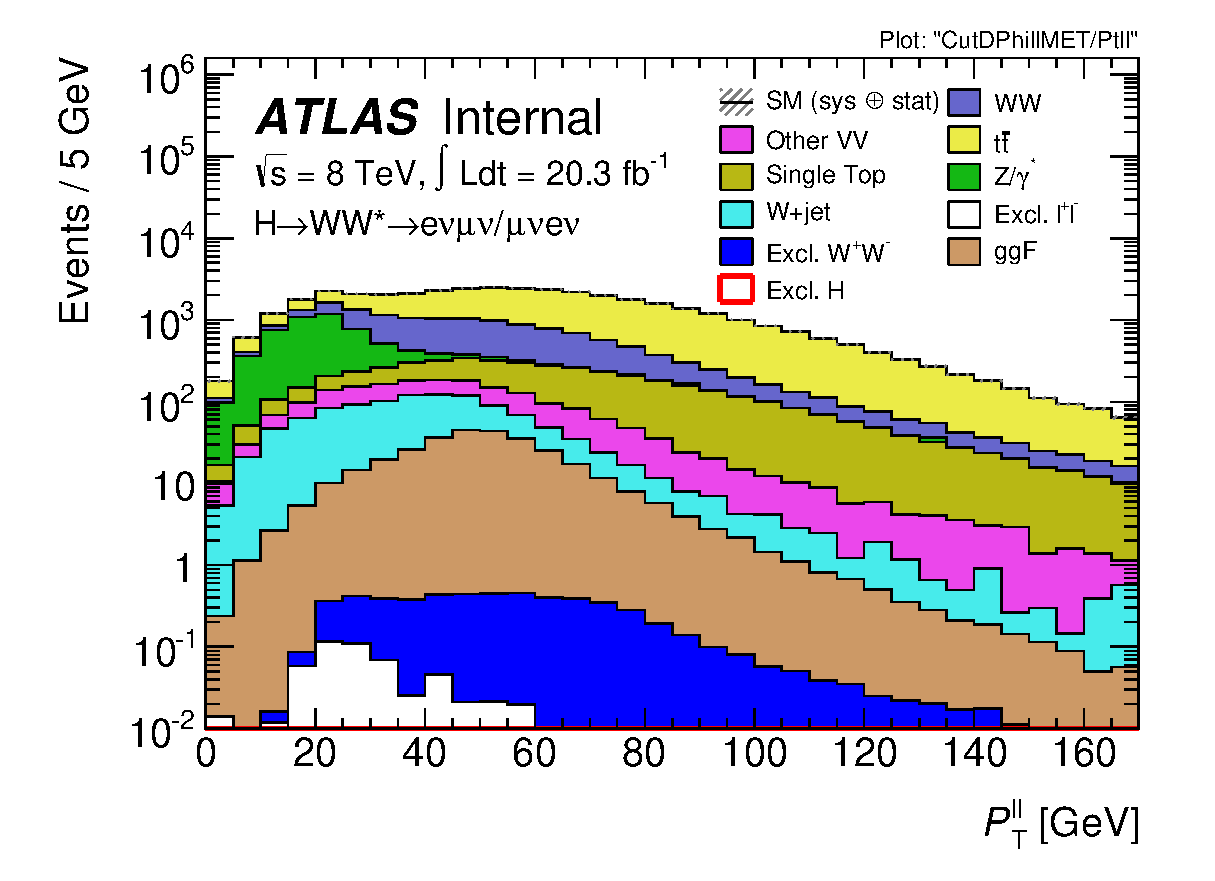
\includegraphics[width=0.5\linewidth]{emme_CutDPhillMET_Ptll_mh125_log.eps}\\
\caption{ptll}
\label{fig:ptll}
\end{figure}

\par talk about dphill and add a plot
\begin{figure}[!h]
\centering
	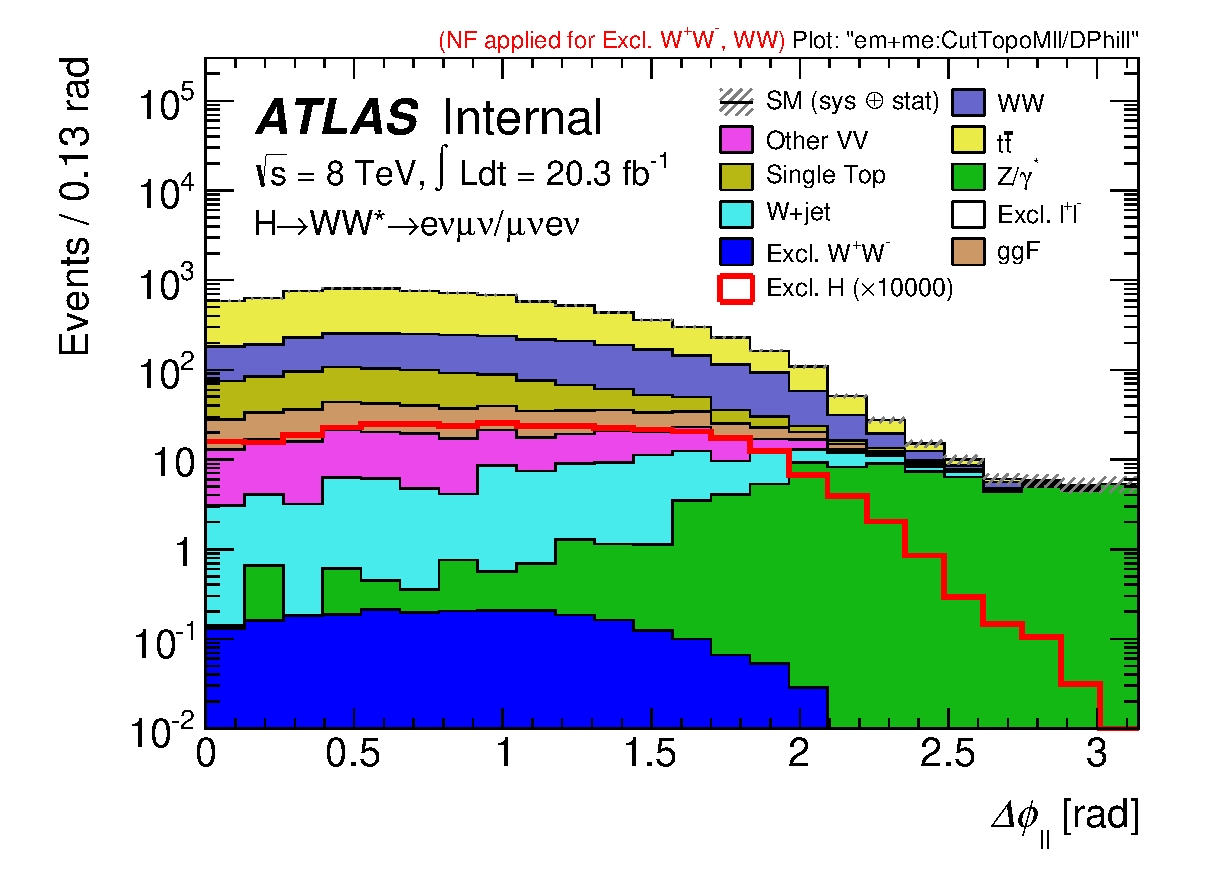
\includegraphics[width=0.5\linewidth]{emme_CutTopoMll_DPhill_mh125_log.eps}\\
\caption{dphill}
\label{fig:dphill}
\end{figure}

\begin{table}
\begin{center}
        \resizebox{0.9\textwidth}{!}{
\begin{tabular}{l||rrrr}
Cut & Excl. H & ggF H & $WW$ & Excl. $W^{+}W^{-}$ \\
\hline\hline
\textcolor{blue}{Scale factors} & \color{blue}NF = 100.00 &  &  &  \\
 blinding & 6.99 $\pm$ 0.05 & 585.63 $\pm$ 1.00 & 11641.95 $\pm$ 18.53 & 6.49 $\pm$ 0.03 \\
lepton $p_{\mathrm{T}}$ 25, 15 GeV & 4.59 $\pm$ 0.04 & 434.84 $\pm$ 0.86 & 10657.89 $\pm$ 17.79 & 5.84 $\pm$ 0.03 \\
OS leptons & 4.59 $\pm$ 0.04 & 434.23 $\pm$ 0.86 & 10618.52 $\pm$ 17.76 & 5.82 $\pm$ 0.03 \\
$m_{\ell\ell} > 10$ GeV & 4.52 $\pm$ 0.04 & 430.02 $\pm$ 0.86 & 10606.74 $\pm$ 17.75 & 5.82 $\pm$ 0.03 \\
$E^{\mathrm{miss}}_{\mathrm{T,rel}} > 25$ GeV & 4.27 $\pm$ 0.04 & 358.80 $\pm$ 0.78 & 8494.57 $\pm$ 15.88 & 5.23 $\pm$ 0.03 \\
$\Delta\phi_{\ell\ell, MET} > 1.57$ & 4.27 $\pm$ 0.04 & 318.16 $\pm$ 0.74 & 7590.42 $\pm$ 15.01 & 5.22 $\pm$ 0.03 \\
$p_{\mathrm{T},\ell\ell}>$30 GeV & 3.83 $\pm$ 0.04 & 285.01 $\pm$ 0.70 & 6183.69 $\pm$ 13.54 & 4.63 $\pm$ 0.03 \\
$m_{\ell\ell}<55$ GeV & 3.28 $\pm$ 0.03 & 246.08 $\pm$ 0.65 & 1578.43 $\pm$ 6.80 & 0.81 $\pm$ 0.01 \\
$\Delta\phi_{\ell\ell}<1.8$ & 2.98 $\pm$ 0.03 & 231.26 $\pm$ 0.63 & 1462.57 $\pm$ 6.54 & 0.77 $\pm$ 0.01 \\
\hline
Exclusivity Cuts & & & &
\end{tabular}
}
\caption{Yields are normalized to 20.3\ifb. Define 'Blinding'}
\end{center}
\end{table}
